\documentclass[]{article}
\usepackage{lmodern}
\usepackage{amssymb,amsmath}
\usepackage{ifxetex,ifluatex}
\usepackage{fixltx2e} % provides \textsubscript
\ifnum 0\ifxetex 1\fi\ifluatex 1\fi=0 % if pdftex
  \usepackage[T1]{fontenc}
  \usepackage[utf8]{inputenc}
\else % if luatex or xelatex
  \ifxetex
    \usepackage{mathspec}
  \else
    \usepackage{fontspec}
  \fi
  \defaultfontfeatures{Ligatures=TeX,Scale=MatchLowercase}
\fi
% use upquote if available, for straight quotes in verbatim environments
\IfFileExists{upquote.sty}{\usepackage{upquote}}{}
% use microtype if available
\IfFileExists{microtype.sty}{%
\usepackage{microtype}
\UseMicrotypeSet[protrusion]{basicmath} % disable protrusion for tt fonts
}{}
\usepackage[margin=1in]{geometry}
\usepackage{hyperref}
\PassOptionsToPackage{usenames,dvipsnames}{color} % color is loaded by hyperref
\hypersetup{unicode=true,
            pdftitle={README for the classification tree},
            pdfauthor={Group 2},
            colorlinks=true,
            linkcolor=Maroon,
            citecolor=Blue,
            urlcolor=blue,
            breaklinks=true}
\urlstyle{same}  % don't use monospace font for urls
\usepackage{longtable,booktabs}
\usepackage{graphicx,grffile}
\makeatletter
\def\maxwidth{\ifdim\Gin@nat@width>\linewidth\linewidth\else\Gin@nat@width\fi}
\def\maxheight{\ifdim\Gin@nat@height>\textheight\textheight\else\Gin@nat@height\fi}
\makeatother
% Scale images if necessary, so that they will not overflow the page
% margins by default, and it is still possible to overwrite the defaults
% using explicit options in \includegraphics[width, height, ...]{}
\setkeys{Gin}{width=\maxwidth,height=\maxheight,keepaspectratio}
\IfFileExists{parskip.sty}{%
\usepackage{parskip}
}{% else
\setlength{\parindent}{0pt}
\setlength{\parskip}{6pt plus 2pt minus 1pt}
}
\setlength{\emergencystretch}{3em}  % prevent overfull lines
\providecommand{\tightlist}{%
  \setlength{\itemsep}{0pt}\setlength{\parskip}{0pt}}
\setcounter{secnumdepth}{0}
% Redefines (sub)paragraphs to behave more like sections
\ifx\paragraph\undefined\else
\let\oldparagraph\paragraph
\renewcommand{\paragraph}[1]{\oldparagraph{#1}\mbox{}}
\fi
\ifx\subparagraph\undefined\else
\let\oldsubparagraph\subparagraph
\renewcommand{\subparagraph}[1]{\oldsubparagraph{#1}\mbox{}}
\fi

%%% Use protect on footnotes to avoid problems with footnotes in titles
\let\rmarkdownfootnote\footnote%
\def\footnote{\protect\rmarkdownfootnote}

%%% Change title format to be more compact
\usepackage{titling}

% Create subtitle command for use in maketitle
\providecommand{\subtitle}[1]{
  \posttitle{
    \begin{center}\large#1\end{center}
    }
}

\setlength{\droptitle}{-2em}

  \title{README for the classification tree}
    \pretitle{\vspace{\droptitle}\centering\huge}
  \posttitle{\par}
    \author{Group 2}
    \preauthor{\centering\large\emph}
  \postauthor{\par}
      \predate{\centering\large\emph}
  \postdate{\par}
    \date{\texttt{December,\ 2nd,\ 2019}}


\begin{document}
\maketitle
\begin{abstract}
This Chapter is describes the classification tree algorithm applied to
the different data sets (all with '\_3', one unsampled and four
sampled), coded in the script `ClassificationTree.R'.
\end{abstract}

\hypertarget{fundamentals-of-classification-trees}{%
\subsection{Fundamentals of Classification
Trees}\label{fundamentals-of-classification-trees}}

Classification trees split the different variables in order to obtain
the most homogeneos possible clusters, by minimizing a loss function,
that can be restricted (this complexity parameter is called `cp' in the
rpart-Package). For every split it computes the sum of the errors on
both sides of the split for all Variables and chooses the one with the
lowest error.

\hypertarget{our-approach}{%
\subsection{Our Approach}\label{our-approach}}

As also applied in the other models, we use all the available
information just before the 2014 NFL-Draft, in order to train the model
and then apply it on the data for 2014. In other words we act as if it
was the end of April 2014 (which is one week before the draft).

For growing trees on our College League / NFL Draft data, we check
whether the best results can be optained, by manually splitting the data
sets on the three postitions (QB / WR / RB) or if the computer will do
that on his own. For growing the trees we use the rpart-Package, which
is commonly used for this purpose, since it does very much on his own.
When growing a tree it uses k-fold cross-validation (by default k=10)
for optimizing the model with respect to the best complexity and the
spots to split. Therefore we do no further cross-validation on the data
set.

You can see the different trees, that we grew, plotted with the
fancyRpartPlot-function out of the rattle-Package in the Appendix at the
end of this file. We are cross-validating the sampling methods and
therefore grow 20 trees in total, we will still just display the four
trees from the unsampled dataframe. Since we use data with many
variables and a couple of splits are made, the plots are not really
readable. The aim of showing them, is to visualize the complexity of the
trees.

\hypertarget{performance-measurement-of-the-trees}{%
\subsection{Performance Measurement of the
trees}\label{performance-measurement-of-the-trees}}

We now want to have a look on the performance of the trees. In order to
compare the results to other models performance, we decided to always
take unsampled data for this. And since our business case is to predict
the 2014 draft (as if it was the day before), we apply it on the data
from 2007 to 2013 to compare the classification errors.

\begin{longtable}[]{@{}lrrrrr@{}}
\caption{True Positives/Negatives and False Positives/Negatives of the
trees for the different models}\tabularnewline
\toprule
& No Sampling & Oversampling & Undersampling & Rose Both &
Smote\tabularnewline
\midrule
\endfirsthead
\toprule
& No Sampling & Oversampling & Undersampling & Rose Both &
Smote\tabularnewline
\midrule
\endhead
QB\_TP & 46 & 68 & 70 & 65 & 65\tabularnewline
QB\_TN & 327 & 292 & 221 & 276 & 281\tabularnewline
QB\_FP & 10 & 45 & 116 & 61 & 56\tabularnewline
QB\_FN & 27 & 5 & 3 & 8 & 8\tabularnewline
WR\_TP & 79 & 146 & 152 & 149 & 138\tabularnewline
WR\_TN & 1118 & 948 & 921 & 889 & 910\tabularnewline
WR\_FP & 18 & 188 & 215 & 247 & 226\tabularnewline
WR\_FN & 85 & 18 & 12 & 15 & 26\tabularnewline
RB\_TP & 48 & 80 & 74 & 81 & 81\tabularnewline
RB\_TN & 527 & 462 & 437 & 425 & 412\tabularnewline
RB\_FP & 11 & 76 & 101 & 113 & 126\tabularnewline
RB\_FN & 42 & 10 & 16 & 9 & 9\tabularnewline
Together\_TP & 116 & 291 & 290 & 289 & 271\tabularnewline
Together\_TN & 1974 & 1563 & 1566 & 1522 & 1599\tabularnewline
Together\_FP & 37 & 448 & 445 & 489 & 412\tabularnewline
Together\_FN & 211 & 36 & 37 & 38 & 56\tabularnewline
\bottomrule
\end{longtable}

In order to compare them better, we will now have a look at the ratio of
correct classification, which is equal to:

\begin{center}
$\frac{Correct Classifications}{All Classifications} = \frac{TP + TN}{TP+TP+FP+FN}$
\end{center}

\begin{longtable}[]{@{}lrrrr@{}}
\caption{Percentage of right classifications}\tabularnewline
\toprule
Sampling & QB & WR & RB & Together\tabularnewline
\midrule
\endfirsthead
\toprule
Sampling & QB & WR & RB & Together\tabularnewline
\midrule
\endhead
no\_sampling & 0.9098 & 0.9208 & 0.9156 & 0.8939\tabularnewline
oversampling & 0.8780 & 0.8415 & 0.8631 & 0.7930\tabularnewline
undersampling & 0.7098 & 0.8254 & 0.8137 & 0.7938\tabularnewline
Rose\_both & 0.8317 & 0.7985 & 0.8057 & 0.7746\tabularnewline
Smote & 0.8439 & 0.8062 & 0.7850 & 0.7998\tabularnewline
\bottomrule
\end{longtable}

\hypertarget{conclusion}{%
\subsection{Conclusion}\label{conclusion}}

As we see, the models for the manually separated positions mostly
perform better than the model for QB/WR/RB together. But the bigger
effect, which we can see, is that the sampling reduces the accuracy of
the models quite much. Since we have 12.4\% of drafted players in the
data, a model predicting 0 (=not drafted) would outperform the models
trained on sampled data.

Within the Classification tree models, the highest accuracy could be
obtained, by using the three models for the manually separated positions
with a weighted average accuracy of 91.74\%. Keeping in mind, that a
model that always predicts `0' would also have an accuracy of 87.6\%,
this models performance, which looks very good on the first sight, is
only a quite small improvement.

\hypertarget{appendix}{%
\subsection{Appendix}\label{appendix}}

\begin{figure}
\hypertarget{id}{%
\centering
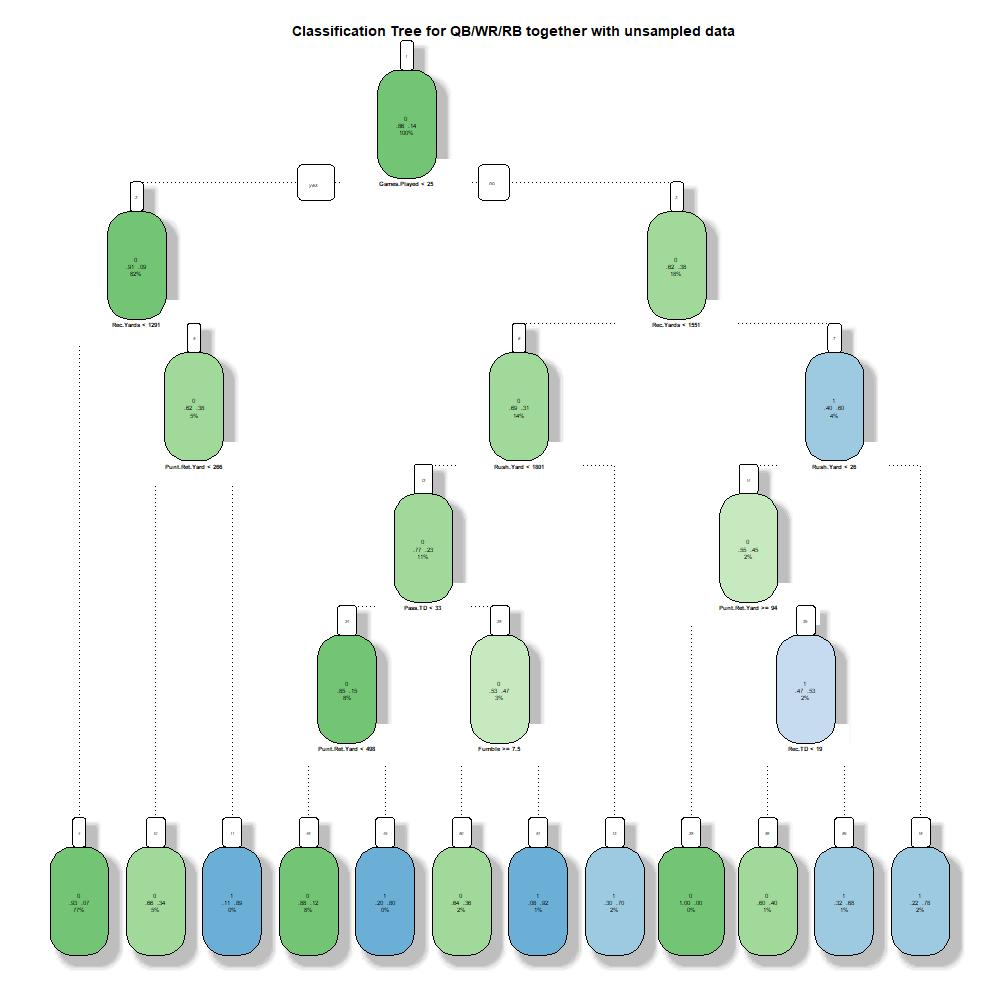
\includegraphics[width=0.5\textwidth,height=\textheight]{../../Project_Scripts/TogethertreeNS.jpg}
\caption{Tree for QB/WR/RB together on unsampled data}\label{id}
}
\end{figure}

\begin{figure}
\hypertarget{id}{%
\centering
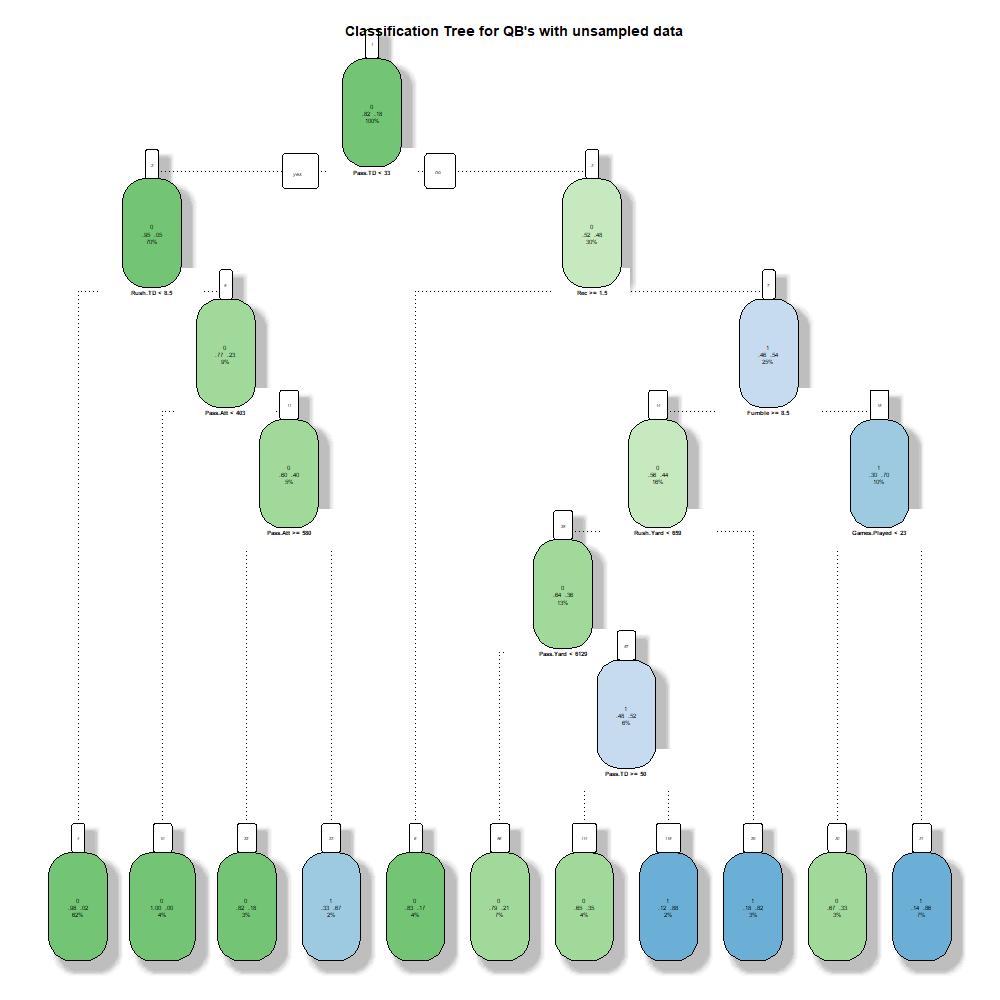
\includegraphics[width=0.5\textwidth,height=\textheight]{../../Project_Scripts/QBtreeNS.jpg}
\caption{Tree for QB's on unsampled data}\label{id}
}
\end{figure}

\begin{figure}
\hypertarget{id}{%
\centering
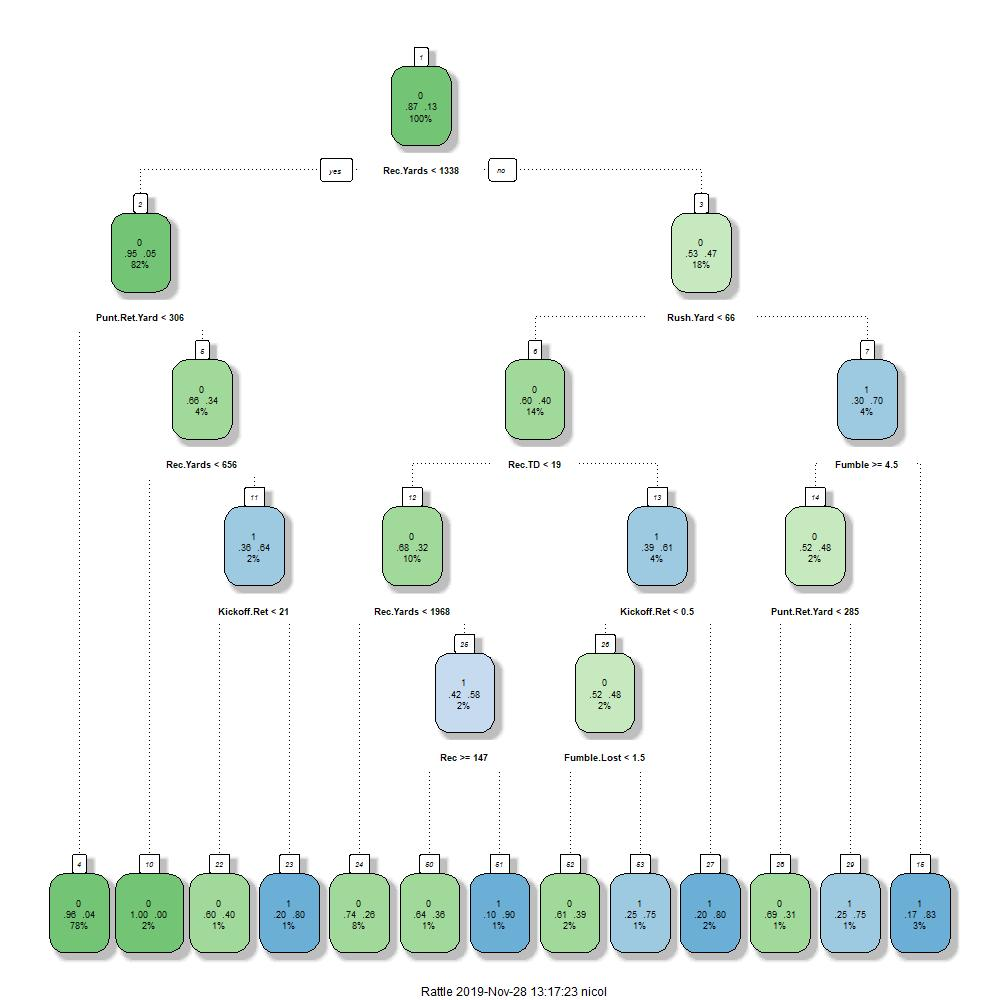
\includegraphics[width=0.5\textwidth,height=\textheight]{../../Project_Scripts/WRtreeNS.jpg}
\caption{Tree for WR's on unsampled data}\label{id}
}
\end{figure}

\begin{figure}
\hypertarget{id}{%
\centering
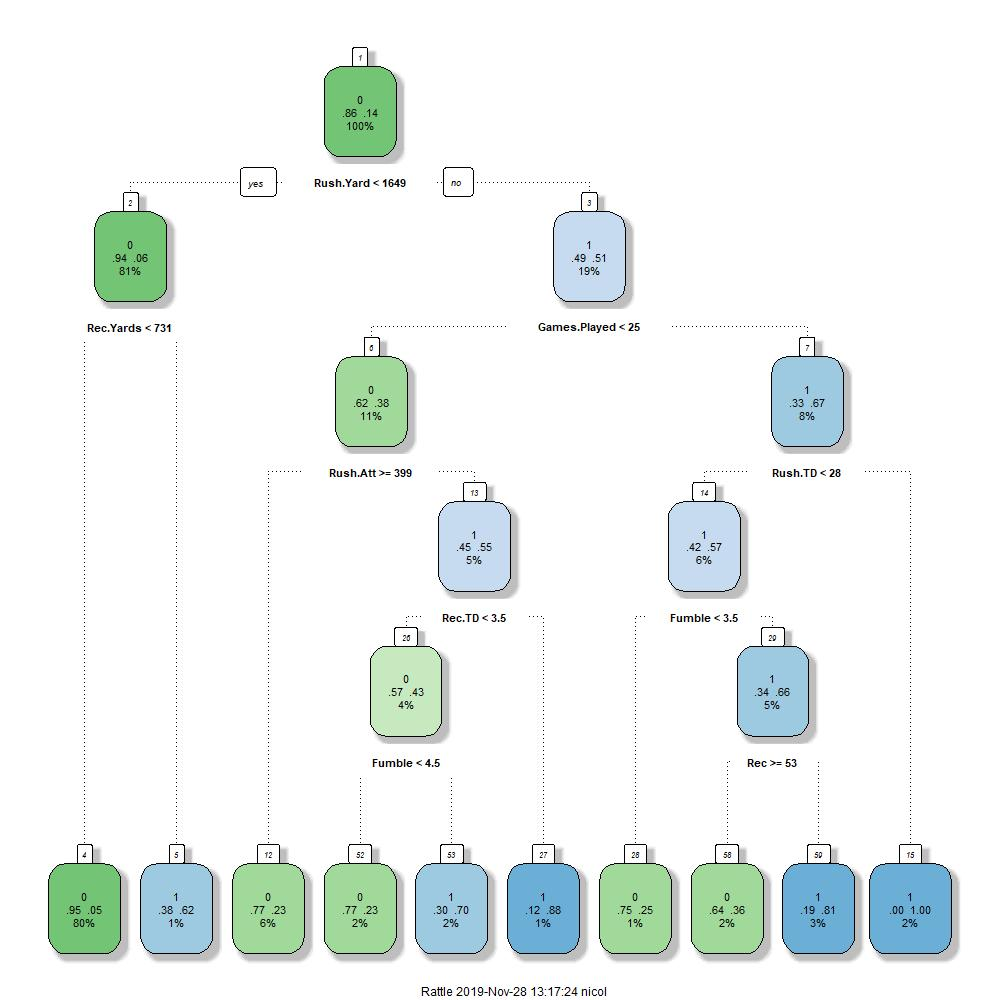
\includegraphics[width=0.5\textwidth,height=\textheight]{../../Project_Scripts/RBtreeNS.jpg}
\caption{Tree for RB's on unsampled data}\label{id}
}
\end{figure}


\end{document}
